\begin{figure}[H]
    \centering
    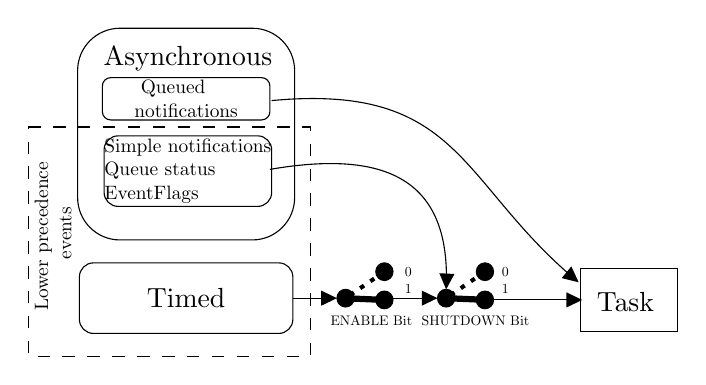
\begin{tikzpicture}[x=0.75pt,y=0.75pt,yscale=-0.85,xscale=0.85]
        \draw   (41.5,194) .. controls (41.5,189.58) and (45.08,186) .. (49.5,186) -- (154.5,186) .. controls (158.92,186) and (162.5,189.58) .. (162.5,194) -- (162.5,218) .. controls (162.5,222.42) and (158.92,226) .. (154.5,226) -- (49.5,226) .. controls (45.08,226) and (41.5,222.42) .. (41.5,218) -- cycle ;
        \draw   (40.5,77) .. controls (40.5,63.75) and (51.25,53) .. (64.5,53) -- (139.5,53) .. controls (152.75,53) and (163.5,63.75) .. (163.5,77) -- (163.5,149) .. controls (163.5,162.25) and (152.75,173) .. (139.5,173) -- (64.5,173) .. controls (51.25,173) and (40.5,162.25) .. (40.5,149) -- cycle ;
        \draw   (55.5,122) .. controls (55.5,117.58) and (59.08,114) .. (63.5,114) -- (142.5,114) .. controls (146.92,114) and (150.5,117.58) .. (150.5,122) -- (150.5,146) .. controls (150.5,150.42) and (146.92,154) .. (142.5,154) -- (63.5,154) .. controls (59.08,154) and (55.5,150.42) .. (55.5,146) -- cycle ;
        \draw   (325.5,189) -- (380.5,189) -- (380.5,225) -- (325.5,225) -- cycle ;
        \draw [line width=2.25]    (214.38,207) -- (191,206) ;
        \draw  [fill={rgb, 255:red, 0; green, 0; blue, 0 }  ,fill opacity=1 ] (187.5,206) .. controls (187.5,203.24) and (189.68,201) .. (192.38,201) .. controls (195.07,201) and (197.25,203.24) .. (197.25,206) .. controls (197.25,208.76) and (195.07,211) .. (192.38,211) .. controls (189.68,211) and (187.5,208.76) .. (187.5,206) -- cycle ;
        \draw    (324.5,207) -- (276.25,207) ;
        \draw [shift={(326.5,207)}, rotate = 180] [fill={rgb, 255:red, 0; green, 0; blue, 0 }  ][line width=0.75]  [draw opacity=0] (8.93,-4.29) -- (0,0) -- (8.93,4.29) -- cycle    ;
        \draw  [fill={rgb, 255:red, 0; green, 0; blue, 0 }  ,fill opacity=1 ] (209.5,191) .. controls (209.5,188.24) and (211.68,186) .. (214.38,186) .. controls (217.07,186) and (219.25,188.24) .. (219.25,191) .. controls (219.25,193.76) and (217.07,196) .. (214.38,196) .. controls (211.68,196) and (209.5,193.76) .. (209.5,191) -- cycle ;
        \draw  [fill={rgb, 255:red, 0; green, 0; blue, 0 }  ,fill opacity=1 ] (209.5,207) .. controls (209.5,204.24) and (211.68,202) .. (214.38,202) .. controls (217.07,202) and (219.25,204.24) .. (219.25,207) .. controls (219.25,209.76) and (217.07,212) .. (214.38,212) .. controls (211.68,212) and (209.5,209.76) .. (209.5,207) -- cycle ;
        \draw    (185.5,206) -- (162.5,206) ;
        \draw [shift={(187.5,206)}, rotate = 180] [fill={rgb, 255:red, 0; green, 0; blue, 0 }  ][line width=0.75]  [draw opacity=0] (8.93,-4.29) -- (0,0) -- (8.93,4.29) -- cycle    ;
        \draw  [fill={rgb, 255:red, 0; green, 0; blue, 0 }  ,fill opacity=1 ] (244.5,206) .. controls (244.5,203.24) and (246.68,201) .. (249.38,201) .. controls (252.07,201) and (254.25,203.24) .. (254.25,206) .. controls (254.25,208.76) and (252.07,211) .. (249.38,211) .. controls (246.68,211) and (244.5,208.76) .. (244.5,206) -- cycle ;
        \draw  [fill={rgb, 255:red, 0; green, 0; blue, 0 }  ,fill opacity=1 ] (266.5,191) .. controls (266.5,188.24) and (268.68,186) .. (271.38,186) .. controls (274.07,186) and (276.25,188.24) .. (276.25,191) .. controls (276.25,193.76) and (274.07,196) .. (271.38,196) .. controls (268.68,196) and (266.5,193.76) .. (266.5,191) -- cycle ;
        \draw  [color={rgb, 255:red, 0; green, 0; blue, 0 }  ,draw opacity=1 ][fill={rgb, 255:red, 0; green, 0; blue, 0 }  ,fill opacity=1 ] (266.5,207) .. controls (266.5,204.24) and (268.68,202) .. (271.38,202) .. controls (274.07,202) and (276.25,204.24) .. (276.25,207) .. controls (276.25,209.76) and (274.07,212) .. (271.38,212) .. controls (268.68,212) and (266.5,209.76) .. (266.5,207) -- cycle ;
        \draw    (242.5,206) -- (219.5,206) ;
        \draw [shift={(244.5,206)}, rotate = 180] [fill={rgb, 255:red, 0; green, 0; blue, 0 }  ][line width=0.75]  [draw opacity=0] (8.93,-4.29) -- (0,0) -- (8.93,4.29) -- cycle    ;
        \draw    (149.5,133) .. controls (212.86,122.11) and (251.72,136.7) .. (249.46,199.09) ;
        \draw [shift={(249.38,201)}, rotate = 272.8] [fill={rgb, 255:red, 0; green, 0; blue, 0 }  ][line width=0.75]  [draw opacity=0] (8.93,-4.29) -- (0,0) -- (8.93,4.29) -- cycle    ;
        \draw   (54.5,85.8) .. controls (54.5,83.15) and (56.65,81) .. (59.3,81) -- (144.7,81) .. controls (147.35,81) and (149.5,83.15) .. (149.5,85.8) -- (149.5,100.2) .. controls (149.5,102.85) and (147.35,105) .. (144.7,105) -- (59.3,105) .. controls (56.65,105) and (54.5,102.85) .. (54.5,100.2) -- cycle ;
        \draw    (150.5,94) .. controls (257.96,84.05) and (256.52,140.43) .. (323.49,196.16) ;
        \draw [shift={(324.5,197)}, rotate = 219.47] [fill={rgb, 255:red, 0; green, 0; blue, 0 }  ][line width=0.75]  [draw opacity=0] (8.93,-4.29) -- (0,0) -- (8.93,4.29) -- cycle    ;
        \draw  [dash pattern={on 4.5pt off 4.5pt}] (12.5,109) -- (172.5,109) -- (172.5,239) -- (12.5,239) -- cycle ;
        \draw [line width=2.25]    (272.75,207) -- (249.38,206) ;
        \draw [line width=1.5]  [dash pattern={on 1.69pt off 2.76pt}]  (214.38,191) -- (192.38,206) ;
        \draw [line width=1.5]  [dash pattern={on 1.69pt off 2.76pt}]  (271.38,191) -- (249.38,206) ;
        \draw (102,206) node  [align=left] {Timed};
        \draw (103,70) node  [align=left] {Asynchronous};
        \draw (351,208) node  [align=left] {Task};
        \draw (103,134) node [scale=0.7] [align=left] {Simple notifications\\Queue status\\EventFlags};
        \draw (102,93) node [scale=0.7] [align=left] { \ Queued \\notifications};
        \draw (207,219) node [scale=0.5] [align=left] {ENABLE Bit};
        \draw (266,219) node [scale=0.5] [align=left] {SHUTDOWN Bit};
        \draw (26.5,171) node [scale=0.7,rotate=-270] [align=left] {Lower precedence\\ \ \ \ \ \ \ \ \ events};
        \draw (228,196) node [scale=0.5] [align=left] {0\\1};
        \draw (283,196) node [scale=0.5] [align=left] {0\\1};
    \end{tikzpicture}
    \caption{Event flow according operational states}
    \label{fig:eventflow}
\end{figure}